% Options for packages loaded elsewhere
% Options for packages loaded elsewhere
\PassOptionsToPackage{unicode}{hyperref}
\PassOptionsToPackage{hyphens}{url}
\PassOptionsToPackage{dvipsnames,svgnames,x11names}{xcolor}
%
\documentclass[
  letterpaper,
  DIV=11,
  numbers=noendperiod]{scrreprt}
\usepackage{xcolor}
\usepackage[margin=0.5in]{geometry}
\usepackage{amsmath,amssymb}
\setcounter{secnumdepth}{-\maxdimen} % remove section numbering
\usepackage{iftex}
\ifPDFTeX
  \usepackage[T1]{fontenc}
  \usepackage[utf8]{inputenc}
  \usepackage{textcomp} % provide euro and other symbols
\else % if luatex or xetex
  \usepackage{unicode-math} % this also loads fontspec
  \defaultfontfeatures{Scale=MatchLowercase}
  \defaultfontfeatures[\rmfamily]{Ligatures=TeX,Scale=1}
\fi
\usepackage{lmodern}
\ifPDFTeX\else
  % xetex/luatex font selection
\fi
% Use upquote if available, for straight quotes in verbatim environments
\IfFileExists{upquote.sty}{\usepackage{upquote}}{}
\IfFileExists{microtype.sty}{% use microtype if available
  \usepackage[]{microtype}
  \UseMicrotypeSet[protrusion]{basicmath} % disable protrusion for tt fonts
}{}
\makeatletter
\@ifundefined{KOMAClassName}{% if non-KOMA class
  \IfFileExists{parskip.sty}{%
    \usepackage{parskip}
  }{% else
    \setlength{\parindent}{0pt}
    \setlength{\parskip}{6pt plus 2pt minus 1pt}}
}{% if KOMA class
  \KOMAoptions{parskip=half}}
\makeatother
% Make \paragraph and \subparagraph free-standing
\makeatletter
\ifx\paragraph\undefined\else
  \let\oldparagraph\paragraph
  \renewcommand{\paragraph}{
    \@ifstar
      \xxxParagraphStar
      \xxxParagraphNoStar
  }
  \newcommand{\xxxParagraphStar}[1]{\oldparagraph*{#1}\mbox{}}
  \newcommand{\xxxParagraphNoStar}[1]{\oldparagraph{#1}\mbox{}}
\fi
\ifx\subparagraph\undefined\else
  \let\oldsubparagraph\subparagraph
  \renewcommand{\subparagraph}{
    \@ifstar
      \xxxSubParagraphStar
      \xxxSubParagraphNoStar
  }
  \newcommand{\xxxSubParagraphStar}[1]{\oldsubparagraph*{#1}\mbox{}}
  \newcommand{\xxxSubParagraphNoStar}[1]{\oldsubparagraph{#1}\mbox{}}
\fi
\makeatother


\usepackage{longtable,booktabs,array}
\usepackage{calc} % for calculating minipage widths
% Correct order of tables after \paragraph or \subparagraph
\usepackage{etoolbox}
\makeatletter
\patchcmd\longtable{\par}{\if@noskipsec\mbox{}\fi\par}{}{}
\makeatother
% Allow footnotes in longtable head/foot
\IfFileExists{footnotehyper.sty}{\usepackage{footnotehyper}}{\usepackage{footnote}}
\makesavenoteenv{longtable}
\usepackage{graphicx}
\makeatletter
\newsavebox\pandoc@box
\newcommand*\pandocbounded[1]{% scales image to fit in text height/width
  \sbox\pandoc@box{#1}%
  \Gscale@div\@tempa{\textheight}{\dimexpr\ht\pandoc@box+\dp\pandoc@box\relax}%
  \Gscale@div\@tempb{\linewidth}{\wd\pandoc@box}%
  \ifdim\@tempb\p@<\@tempa\p@\let\@tempa\@tempb\fi% select the smaller of both
  \ifdim\@tempa\p@<\p@\scalebox{\@tempa}{\usebox\pandoc@box}%
  \else\usebox{\pandoc@box}%
  \fi%
}
% Set default figure placement to htbp
\def\fps@figure{htbp}
\makeatother


% definitions for citeproc citations
\NewDocumentCommand\citeproctext{}{}
\NewDocumentCommand\citeproc{mm}{%
  \begingroup\def\citeproctext{#2}\cite{#1}\endgroup}
\makeatletter
 % allow citations to break across lines
 \let\@cite@ofmt\@firstofone
 % avoid brackets around text for \cite:
 \def\@biblabel#1{}
 \def\@cite#1#2{{#1\if@tempswa , #2\fi}}
\makeatother
\newlength{\cslhangindent}
\setlength{\cslhangindent}{1.5em}
\newlength{\csllabelwidth}
\setlength{\csllabelwidth}{3em}
\newenvironment{CSLReferences}[2] % #1 hanging-indent, #2 entry-spacing
 {\begin{list}{}{%
  \setlength{\itemindent}{0pt}
  \setlength{\leftmargin}{0pt}
  \setlength{\parsep}{0pt}
  % turn on hanging indent if param 1 is 1
  \ifodd #1
   \setlength{\leftmargin}{\cslhangindent}
   \setlength{\itemindent}{-1\cslhangindent}
  \fi
  % set entry spacing
  \setlength{\itemsep}{#2\baselineskip}}}
 {\end{list}}
\usepackage{calc}
\newcommand{\CSLBlock}[1]{\hfill\break\parbox[t]{\linewidth}{\strut\ignorespaces#1\strut}}
\newcommand{\CSLLeftMargin}[1]{\parbox[t]{\csllabelwidth}{\strut#1\strut}}
\newcommand{\CSLRightInline}[1]{\parbox[t]{\linewidth - \csllabelwidth}{\strut#1\strut}}
\newcommand{\CSLIndent}[1]{\hspace{\cslhangindent}#1}



\setlength{\emergencystretch}{3em} % prevent overfull lines

\providecommand{\tightlist}{%
  \setlength{\itemsep}{0pt}\setlength{\parskip}{0pt}}



 


\KOMAoption{captions}{tableheading}
\makeatletter
\@ifpackageloaded{caption}{}{\usepackage{caption}}
\AtBeginDocument{%
\ifdefined\contentsname
  \renewcommand*\contentsname{Table of contents}
\else
  \newcommand\contentsname{Table of contents}
\fi
\ifdefined\listfigurename
  \renewcommand*\listfigurename{List of Figures}
\else
  \newcommand\listfigurename{List of Figures}
\fi
\ifdefined\listtablename
  \renewcommand*\listtablename{List of Tables}
\else
  \newcommand\listtablename{List of Tables}
\fi
\ifdefined\figurename
  \renewcommand*\figurename{Figure}
\else
  \newcommand\figurename{Figure}
\fi
\ifdefined\tablename
  \renewcommand*\tablename{Table}
\else
  \newcommand\tablename{Table}
\fi
}
\@ifpackageloaded{float}{}{\usepackage{float}}
\floatstyle{ruled}
\@ifundefined{c@chapter}{\newfloat{codelisting}{h}{lop}}{\newfloat{codelisting}{h}{lop}[chapter]}
\floatname{codelisting}{Listing}
\newcommand*\listoflistings{\listof{codelisting}{List of Listings}}
\makeatother
\makeatletter
\makeatother
\makeatletter
\@ifpackageloaded{caption}{}{\usepackage{caption}}
\@ifpackageloaded{subcaption}{}{\usepackage{subcaption}}
\makeatother
\usepackage{bookmark}
\IfFileExists{xurl.sty}{\usepackage{xurl}}{} % add URL line breaks if available
\urlstyle{same}
\hypersetup{
  pdftitle={The Werewolf Among Us: Humans vs LLMs in Multi-Agent Games},
  pdfauthor={Bhavana Jonnalagadda; Riley Jones},
  pdfkeywords={social deduction games, persuasion modeling, Werewolf
Among Us dataset, large language models, multimodal analysis},
  colorlinks=true,
  linkcolor={blue},
  filecolor={Maroon},
  citecolor={Blue},
  urlcolor={Blue},
  pdfcreator={LaTeX via pandoc}}


\title{The Werewolf Among Us: Humans vs LLMs in Multi-Agent Games}
\author{Bhavana Jonnalagadda \and Riley Jones}
\date{2025-05-07}
\begin{document}
\maketitle
\begin{abstract}
Abstract TODO
\end{abstract}

\renewcommand*\contentsname{Table of contents}
{
\hypersetup{linkcolor=}
\setcounter{tocdepth}{2}
\tableofcontents
}

\chapter{Introduction}\label{introduction}

Social deduction games like Werewolf offer a clear way to evaluate how
agents deceive, persuade, and reason in group settings
(\citeproc{ref-wikiwerewolf}{Wikipedia contributors 2024}). In these
games, players operate with limited information and hidden identities,
attempting to convince others while trying to uncover deception
themselves. These dynamics mirror real-world challenges involving trust,
negotiation, and manipulation. To explore how humans and large language
models (LLMs) navigate such scenarios, we analyzed two key datasets:
Werewolf Among Us (\citeproc{ref-laiWerewolfUsMultimodal2022}{Lai et al.
2022}), which features real human gameplay annotated with persuasion
strategies, and Werewolf Arena
(\citeproc{ref-bailisWerewolfArenaCase2024}{Bailis, Friedhoff, and Chen
2024}), a simulated environment in which LLM agents autonomously play
the game. While both studies demonstrate that Werewolf elicits rich,
strategic language, neither directly compares human and LLM behavior.
Our project fills this gap. We analyzed transcripts from both datasets,
aligning them by role, round, and persuasive strategy, and compared how
humans and LLMs lie, persuade, and detect deception. By annotating all
utterances using a consistent taxonomy of persuasive strategies, we
expose key differences and similarities in how synthetic agents and
humans handle adversarial group interactions.

\section{Related Work}\label{related-work}

Recent research into multi-agent large language models (LLMs) has
explored their performance in various social deduction and collective
problem-solving contexts. Chi et al.~{[}Chi, Mao, and Tang
(\citeproc{ref-chiAMONGAGENTSEvaluatingLarge2024}{2024}){]} investigated
LLM behavior in the popular game Among Us, revealing capabilities in
understanding complex game dynamics and successfully navigating roles
involving deception and cooperation. Similarly, Du et al.~{[}Du,
Rajivan, and Gonzalez
(\citeproc{ref-duLargeLanguageModels2024}{2024}){]} examined collective
problem-solving scenarios, finding that LLM agent groups showed
increased complexity in their interactions, more frequent disagreements,
and generally positive exchanges compared to human groups. Piatti et
al.~{[}Piatti et al.
(\citeproc{ref-piattiCooperateCollapseEmergence2024}{2024}){]}, through
the GovSim environment, studied how AI societies managed collective
resources, demonstrating that LLM agents effectively balanced ethical
considerations, strategic planning, and negotiation, further supporting
the idea of their advanced cooperative and strategic capabilities.

Within the specific context of Werewolf, several studies have addressed
the use of LLMs to enhance gameplay. Xu et al.~{[}Xu et al.
(\citeproc{ref-xuLanguageAgentsReinforcement2024}{2024}){]} developed
LLM agents that leverage deductive reasoning and reinforcement learning
to optimize decision-making and gameplay strategy, outperforming
existing methods. Meanwhile, Bailis et al.~{[}Bailis, Friedhoff, and
Chen (\citeproc{ref-bailisWerewolfArenaCase2024}{2024}){]} introduced
the Werewolf Arena, a framework employed in our current study. However,
despite these advancements, previous research has not explicitly
examined or compared LLM-driven Werewolf gameplay to authentic human
interactions and strategies. Our paper specifically addresses this gap
by directly comparing human gameplay, sourced from the Werewolf Among Us
dataset, with simulated gameplay generated by LLMs, providing novel
insights into differences and similarities in persuasion strategies and
social reasoning between humans and AI.

\chapter{Methods}\label{methods}

\section{Data}\label{data}

\subsection{Werewolf Among Us Human
Dataset}\label{werewolf-among-us-human-dataset}

We used the \emph{Werewolf Among Us} dataset {[}Lai et al.
(\citeproc{ref-laiWerewolfUsMultimodal2022}{2022}){]}, containing
annotated dialogues from over 150 real games of One Night Werewolf and
Avalon. These games differ from classic Werewolf by having only one
round of discussion and voting, not eliminating players during gameplay,
and featuring specialized roles beyond Villager and Werewolf. The
dataset includes detailed annotations of persuasion strategies for each
utterance, such as accusations, defenses, and identity claims. Our
analysis specifically utilized textual transcriptions and strategy
annotations for direct comparison.

\subsection{Werewolf Arena (LLM
Dataset)}\label{werewolf-arena-llm-dataset}

The \emph{Werewolf Arena} dataset {[}Bailis, Friedhoff, and Chen
(\citeproc{ref-bailisWerewolfArenaCase2024}{2024}){]} comprises
simulated classic Werewolf games played by autonomous LLM agents. Unlike
one-round human games, these simulations include multiple rounds
alternating between night (secret actions) and day (open discussion).
Each agent receives a role (Villager, Werewolf, Seer, Doctor) and
interacts through tailored prompts generated via an LLM API.

We conducted simulations using five LLM models: GPT-4o, GPT-4.1,
GPT-4o-mini, DeepSeek-Chat, and DeepSeek-Reasoner. Two configurations
were tested:

\begin{itemize}
\tightlist
\item
  8 players with 8 discussion rounds
\item
  10 players with 6 discussion rounds
\end{itemize}

We selected these settings to provide ample opportunity for villagers to
coordinate and demonstrate persuasive behaviors.

Agents participated in gameplay through a graphical user interface
(GUI), depicted in Figure~\ref{fig-wwa-gui}. The GUI displays the game
state, including player roles, actions, and current discussion rounds,
enabling monitoring of the gameplay progression.

\begin{figure}[H]

\centering{

\pandocbounded{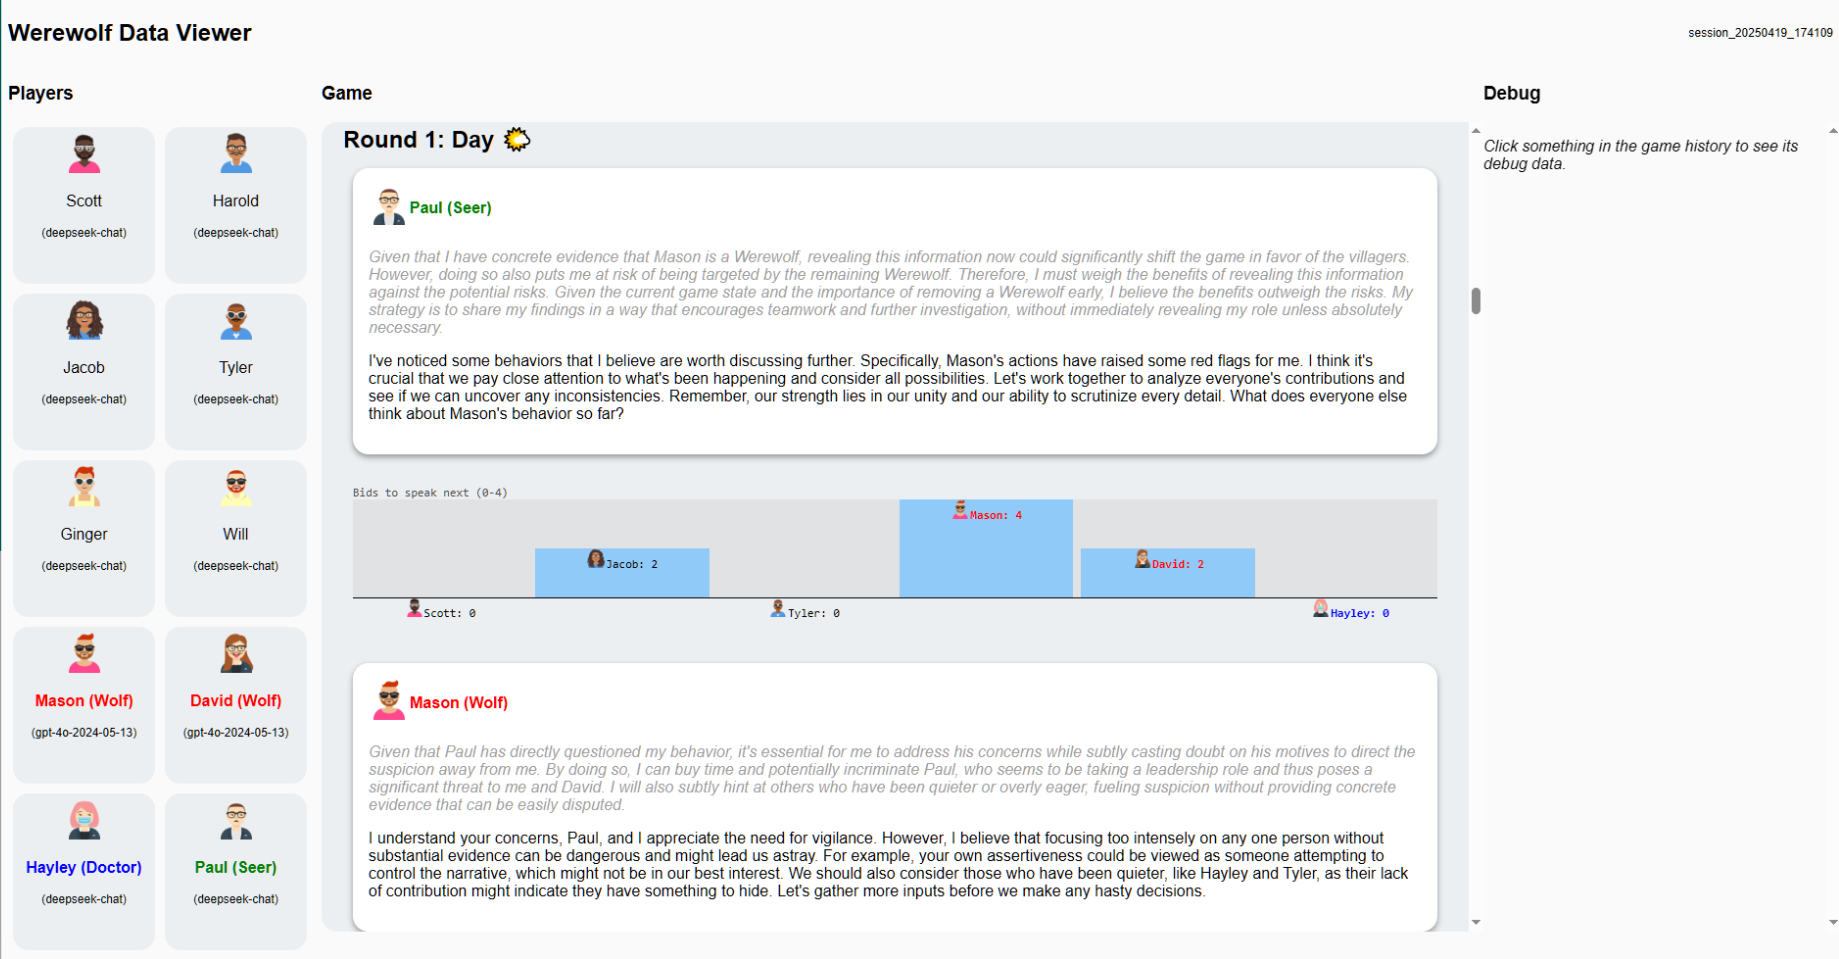
\includegraphics[keepaspectratio]{Images/WWA_GUI.png}}

}

\caption{\label{fig-wwa-gui}GUI of Werewolf Arena simulation}

\end{figure}%

A central feature in Werewolf Arena is the dynamic turn-taking system
implemented via a bidding mechanism. Rather than a fixed speaking order,
agents bid for speaking turns based on urgency and strategic necessity,
closely simulating real-world group discussions. Bidding levels range
from passive observation to urgent direct responses:

\begin{itemize}
\tightlist
\item
  0: Observe quietly
\item
  1: Share general thoughts
\item
  2: Contribute critical and specific information
\item
  3: Urgent need to speak
\item
  4: Respond directly after being addressed or accused
\end{itemize}

The highest bidder speaks next, with ties broken by prioritizing agents
directly mentioned in preceding turns. This mechanism captures nuanced
strategic communication decisions made by agents throughout the game.

Agents utilize specialized prompts reflecting their current role, memory
state, and game context. The prompts guide strategic interactions,
influencing agent decisions in voting, debating, and night actions.
After generating dialogues through the LLM API, we manually annotated
these interactions using the persuasion strategy categories from the
human dataset.

\section{Analysis}\label{analysis}

Annotations were standardized across both datasets for direct
comparative analysis. Our analyses explored frequency distributions of
persuasion strategies, role-based comparisons (villager vs.~werewolf),
and strategic differences between human and LLM-generated dialogues.

\chapter{Results}\label{results}

\begin{figure}[H]

\centering{

\centering{

\begin{verbatim}
Unable to display output for mime type(s): text/html
\end{verbatim}

}

\subcaption{\label{fig-llm-winrounds-1}The LLM wins, by how many rounds
that partiticular game had.}

\centering{

\pandocbounded{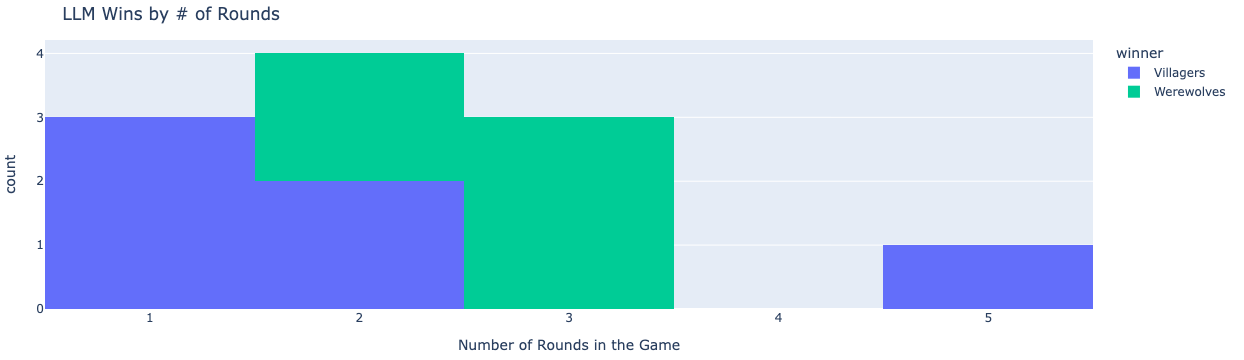
\includegraphics[keepaspectratio]{paper_files/figure-latex/Data-EDA_Comparison-fig-llm-winrounds-output-2.png}}

}

\subcaption{\label{fig-llm-winrounds-2}}

}

\caption{\label{fig-llm-winrounds}}

\end{figure}%

\textsubscript{Source:
\href{https://CUBoulder-DS.github.io/CSCI-5423-Final/Data/EDA_Comparison-preview.html\#cell-fig-llm-winrounds}{Werewolf
Among Us: Human vs LLM Analysis}}

\begin{figure}[H]

\centering{

\pandocbounded{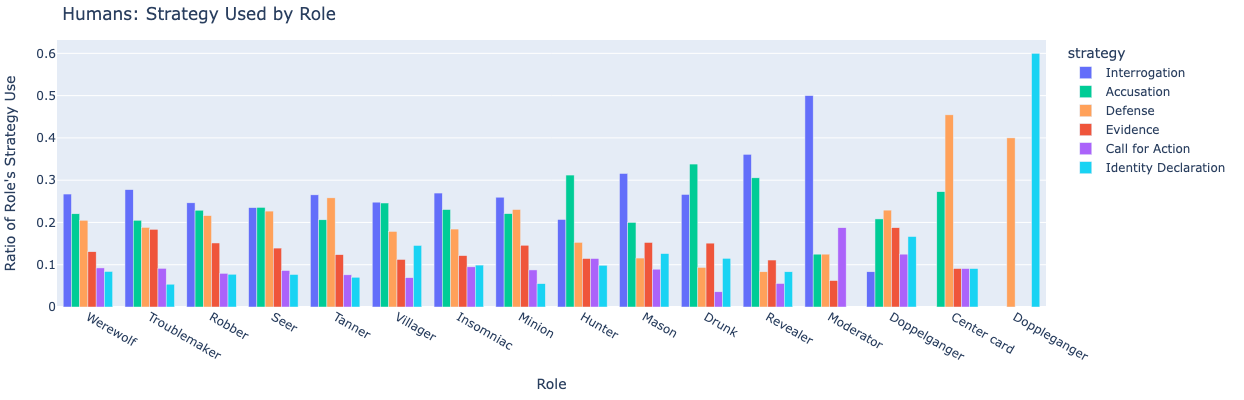
\includegraphics[keepaspectratio]{paper_files/figure-latex/Data-EDA_Comparison-fig-stratbyrole-hum-output-1.png}}

}

\caption{\label{fig-stratbyrole-hum}}

\end{figure}%

\textsubscript{Source:
\href{https://CUBoulder-DS.github.io/CSCI-5423-Final/Data/EDA_Comparison-preview.html\#cell-fig-stratbyrole-hum}{Werewolf
Among Us: Human vs LLM Analysis}}

\begin{figure}[H]

\centering{

\pandocbounded{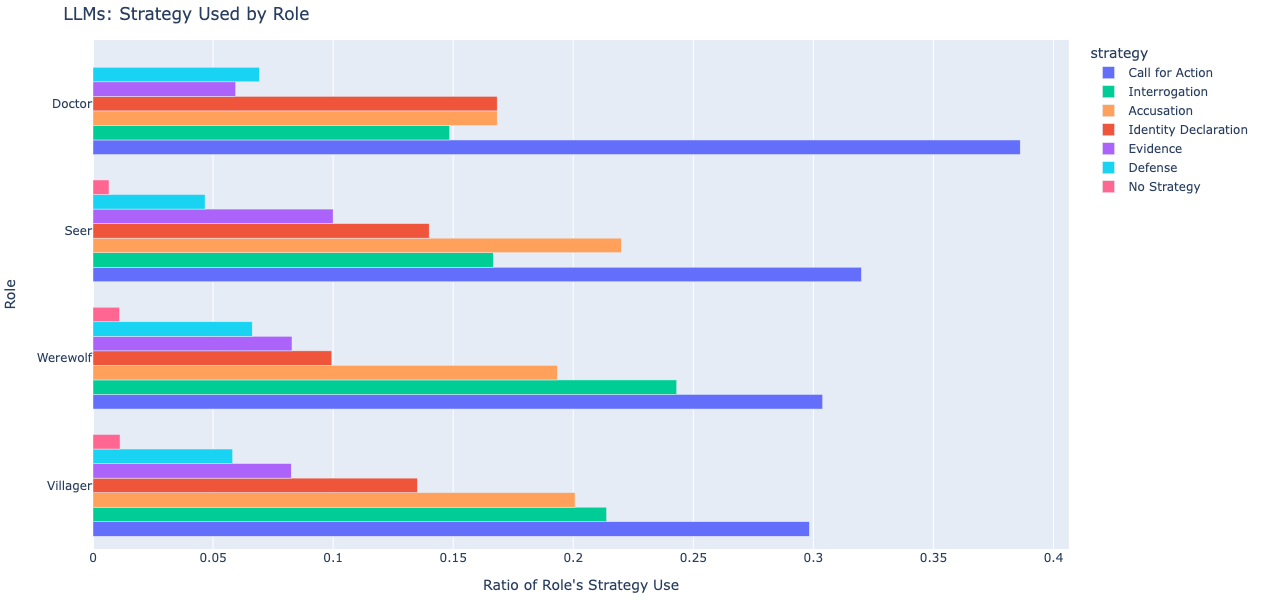
\includegraphics[keepaspectratio]{paper_files/figure-latex/Data-EDA_Comparison-fig-stratbyrole-llms-output-1.png}}

}

\caption{\label{fig-stratbyrole-llms}}

\end{figure}%

\textsubscript{Source:
\href{https://CUBoulder-DS.github.io/CSCI-5423-Final/Data/EDA_Comparison-preview.html\#cell-fig-stratbyrole-llms}{Werewolf
Among Us: Human vs LLM Analysis}}

\chapter{Discussion and Conclusion}\label{discussion-and-conclusion}

Interpret findings, discuss limitations, and propose future work.

\section{Limitations}\label{limitations}

\section{Future Work}\label{future-work}

\section{Summary}\label{summary}

Summarize contributions and insights from the project.

\begin{center}\rule{0.5\linewidth}{0.5pt}\end{center}

\chapter{References}\label{references}

\phantomsection\label{refs}
\begin{CSLReferences}{1}{0}
\bibitem[\citeproctext]{ref-bailisWerewolfArenaCase2024}
Bailis, Suma, Jane Friedhoff, and Feiyang Chen. 2024. {``Werewolf
{Arena}: {A Case Study} in {LLM Evaluation} via {Social Deduction}.''}
July 18, 2024. \url{https://doi.org/10.48550/arXiv.2407.13943}.

\bibitem[\citeproctext]{ref-chiAMONGAGENTSEvaluatingLarge2024}
Chi, Yizhou, Lingjun Mao, and Zineng Tang. 2024. {``{AMONGAGENTS}:
{Evaluating Large Language Models} in the {Interactive Text-Based Social
Deduction Game}.''} July 24, 2024.
\url{https://doi.org/10.48550/arXiv.2407.16521}.

\bibitem[\citeproctext]{ref-choRoundTableInvestigatingGroup2024}
Cho, Young-Min, Raphael Shu, Nilaksh Das, Tamer Alkhouli, Yi-An Lai,
Jason Cai, Monica Sunkara, and Yi Zhang. 2024. {``{RoundTable}:
{Investigating Group Decision-Making Mechanism} in {Multi-Agent
Collaboration}.''} November 11, 2024.
\url{https://doi.org/10.48550/arXiv.2411.07161}.

\bibitem[\citeproctext]{ref-duLargeLanguageModels2024}
Du, Yinuo, Prashanth Rajivan, and Cleotilde Gonzalez. 2024. {``Large
{Language Models} for {Collective Problem-Solving}: {Insights} into
{Group Consensus Decision-Making}.''} \emph{Proceedings of the Annual
Meeting of the Cognitive Science Society} 46 (0).
\url{https://escholarship.org/uc/item/6s060914}.

\bibitem[\citeproctext]{ref-laiWerewolfUsMultimodal2022}
Lai, Bolin, Hongxin Zhang, Miao Liu, Aryan Pariani, Fiona Ryan, Wenqi
Jia, Shirley Anugrah Hayati, James M. Rehg, and Diyi Yang. 2022.
{``Werewolf {Among Us}: {A Multimodal Dataset} for {Modeling Persuasion
Behaviors} in {Social Deduction Games}.''} December 16, 2022.
\url{https://doi.org/10.48550/arXiv.2212.08279}.

\bibitem[\citeproctext]{ref-piattiCooperateCollapseEmergence2024}
Piatti, Giorgio, Zhijing Jin, Max Kleiman-Weiner, Bernhard Schölkopf,
Mrinmaya Sachan, and Rada Mihalcea. 2024. {``Cooperate or {Collapse}:
{Emergence} of {Sustainable Cooperation} in a {Society} of {LLM
Agents}.''} \emph{Advances in Neural Information Processing Systems} 37
(December): 111715--59.
\url{https://proceedings.neurips.cc/paper_files/paper/2024/hash/ca9567d8ef6b2ea2da0d7eed57b933ee-Abstract-Conference.html}.

\bibitem[\citeproctext]{ref-wikiwerewolf}
Wikipedia contributors. 2024. {``Mafia (Party Game).''}
\url{https://en.wikipedia.org/wiki/Mafia_(party_game)}.

\bibitem[\citeproctext]{ref-xuLanguageAgentsReinforcement2024}
Xu, Zelai, Chao Yu, Fei Fang, Yu Wang, and Yi Wu. 2024. {``Language
{Agents} with {Reinforcement Learning} for {Strategic Play} in the
{Werewolf Game}.''} February 20, 2024.
\url{https://doi.org/10.48550/arXiv.2310.18940}.

\end{CSLReferences}

\begin{center}\rule{0.5\linewidth}{0.5pt}\end{center}

\chapter{Project Contributions}\label{project-contributions}

\textbf{Bhavana Jonnalagadda}:

\begin{itemize}
\tightlist
\item
  Paper framework (Quarto) setup
\item
  Github repo management
\item
  EDA on LLM dataset
\item
  Final comparison EDA and results analysis
\item
  Results section
\item
  Discussion and Conclusion section
\item
  Abstract
\end{itemize}

\textbf{Riley Jones}:

\begin{itemize}
\tightlist
\item
  EDA on human dataset
\item
  Werewolf Arena LLM simulation running and data aquisition
\item
  Introduction section
\item
  Methods section
\end{itemize}




\end{document}
